\begin{figure}
  \centering
\begin{subfigure}[b]{0.45\textwidth}
   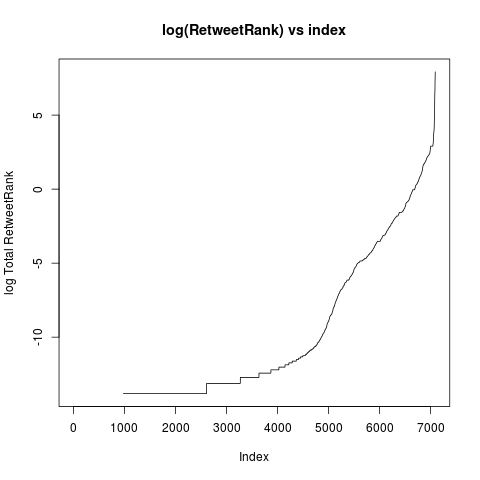
\includegraphics[width=\textwidth]{../src/Analysis/retweetrankcurve.png}
   \caption{The log of the $RR_u$ plotting against its sorted index.}
   \label{fig:rtrate}  
\end{subfigure}%
\begin{subfigure}[b]{0.45\textwidth}
   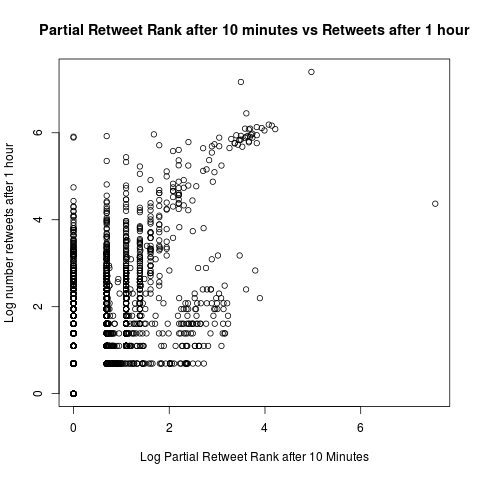
\includegraphics[width=\textwidth]{../src/Analysis/partialrtr.png}
   \caption{The relation between $RR_u^{(10min)}$ and $R_u^{1hr}$}
   \label{fig:partialpair}  
\end{subfigure}
\end{figure}
 \begin{figure}
   \centering
  \begin{subfigure}[b]{0.45\textwidth}
    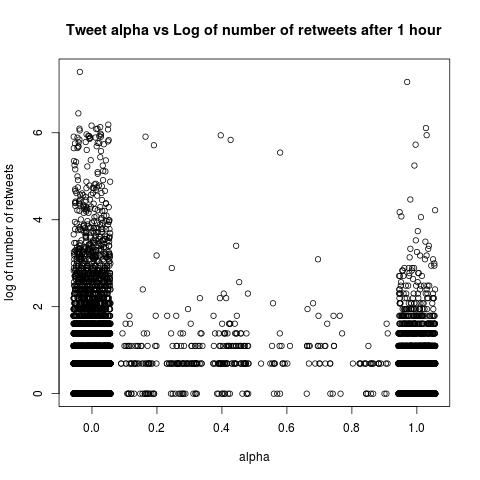
\includegraphics[width=\textwidth]{../src/Analysis/alphadist.png}
    \caption{Total Alpha vs log Retweets}
    \label{fig:gull}
  \end{subfigure}%
  \begin{subfigure}[b]{0.45\textwidth}
    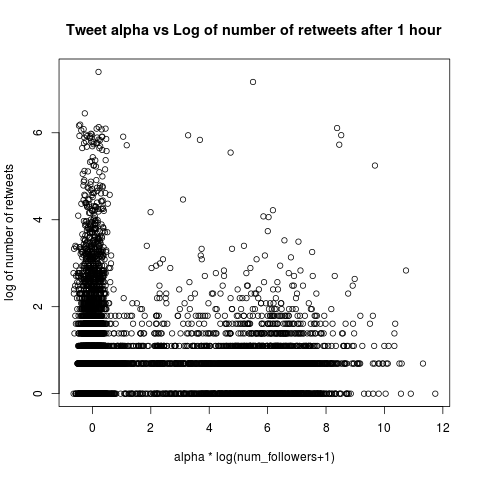
\includegraphics[width=\textwidth]{../src/Analysis/alphalognfdist.png}
    \caption{Total Alpha * log of followers vs log Retweets}
    \label{fig:mouse}
  \end{subfigure}
  \caption{Relation between Alpha and log of Retweets after an hour)}\label{fig:animals}
\end{figure}

\begin{figure}
  \centering
  \begin{subfigure}[b]{0.45\textwidth}
    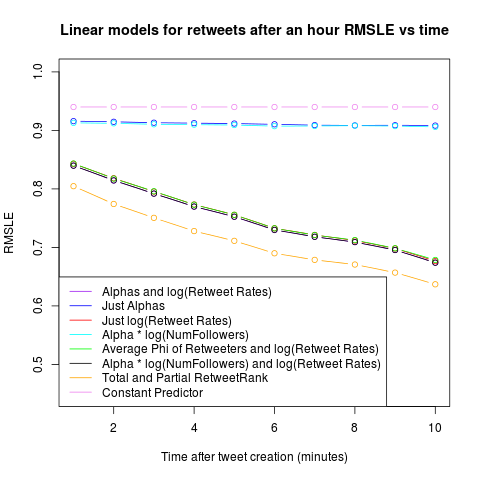
\includegraphics[width=\textwidth]{../src/Analysis/linearattempts.png}
    \caption{Early prediction curves for various features sets\\ using Linear Models}
    \label{fig:linearattempts}  
  \end{subfigure}%
  \begin{subfigure}[b]{0.45\textwidth}
    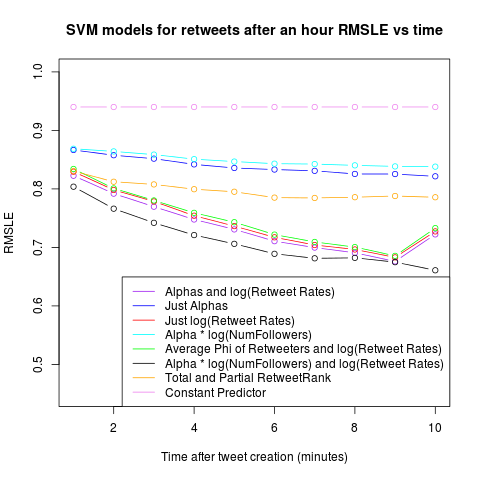
\includegraphics[width=\textwidth]{../src/Analysis/svmattempts.png}
    \caption{Early prediction curves for various features sets\\ using Support Vector Machines}
    \label{fig:svmattempts}  
  \end{subfigure}
  \begin{subfigure}[b]{0.45\textwidth}
    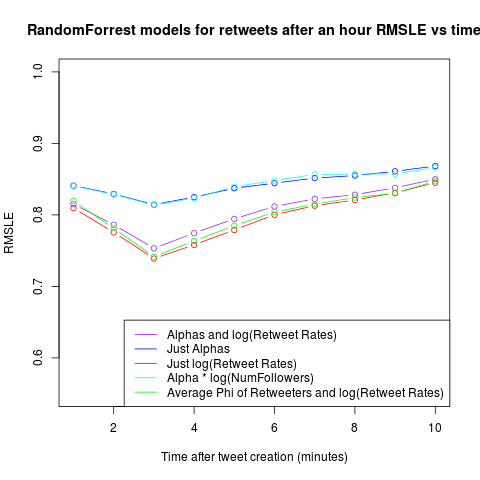
\includegraphics[width=\textwidth]{../src/Analysis/rfattempts.png}
    \caption{Early prediction curves for various features sets \\using Random Forests}
    \label{fig:rfattempts}  
  \end{subfigure}%
  \begin{subfigure}[b]{0.45\textwidth}
    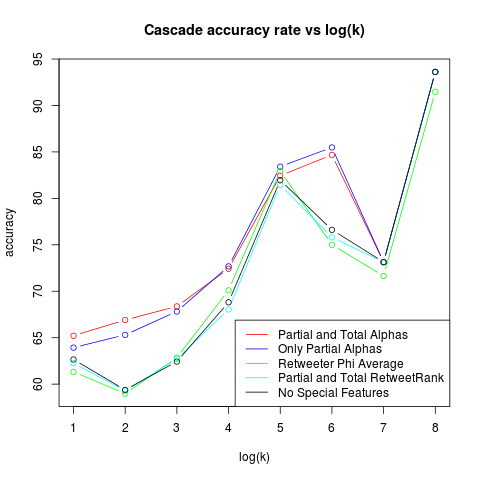
\includegraphics[width=\textwidth]{../src/Analysis/jurerocks.png}
    \caption{Accuracy rates using ``cascading'' experimental setup from \cite{DBLP:journals/corr/ChengADKL14}}
    \label{fig:jurerocks}  
  \end{subfigure}
  \caption{Experimental Prediction Results}
\end{figure}  


